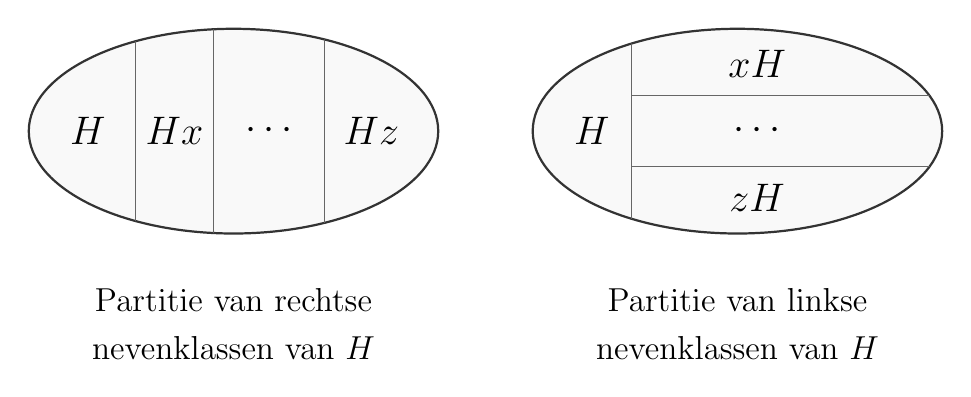
\begin{tikzpicture}[>=latex]

% --- Stijldefinities ---
\tikzset{
    quotientSet/.style={
        fill=gray!5,
        draw=black!80,
        thick
    },
    partitionLine/.style={
        draw=black!60,
        thin
    },
    cosetLabel/.style={
        font=\Large
    },
    captionLabel/.style={
        font=\large,
        align=center
    }
}

% =========================================================
% Linker figuur: Partitie van rechtse nevenklassen
% =========================================================

\draw[quotientSet] (0,0) ellipse (2.6cm and 1.3cm);

% Verticale scheidingslijnen binnen de ellips
\begin{scope}
    \clip (0,0) ellipse (2.6cm and 1.3cm);
    \draw[partitionLine] (-1.25,-1.5) -- (-1.25,1.5);
    \draw[partitionLine] (-0.25,-1.5) -- (-0.25,1.5);
    \draw[partitionLine] (1.15,-1.5) -- (1.15,1.5);
\end{scope}

% Labels
\node[cosetLabel] at (-1.85,0) {$H$};
\node[cosetLabel] at (-0.75,0) {$Hx$};
\node[cosetLabel] at (0.45,0) {$\cdots$};
\node[cosetLabel] at (1.75,0) {$Hz$};

% Onderschrift
\node[captionLabel] at (0,-2.15) {Partitie van rechtse};
\node[captionLabel] at (0,-2.75) {nevenklassen van $H$};


% =========================================================
% Rechter figuur: Partitie van linkse nevenklassen
% =========================================================

\begin{scope}[xshift=6.4cm]

\draw[quotientSet] (0,0) ellipse (2.6cm and 1.3cm);

% Scheidingslijnen binnen de ellips
\begin{scope}
    \clip (0,0) ellipse (2.6cm and 1.3cm);

    % Verticale lijn die H afscheidt
    \draw[partitionLine] (-1.35,-1.5) -- (-1.35,1.5);

    % Horizontale lijnen voor xH, ..., zH
    \draw[partitionLine] (-1.35,0.45) -- (3,0.45);
    \draw[partitionLine] (-1.35,-0.45) -- (3,-0.45);
\end{scope}

% Labels
\node[cosetLabel] at (-1.85,0) {$H$};
\node[cosetLabel] at (0.25,0.85) {$xH$};
\node[cosetLabel] at (0.25,0) {$\cdots$};
\node[cosetLabel] at (0.25,-0.85) {$zH$};

% Onderschrift
\node[captionLabel] at (0,-2.15) {Partitie van linkse};
\node[captionLabel] at (0,-2.75) {nevenklassen van $H$};

\end{scope}

\end{tikzpicture}